\chapter{Tensor-based Discriminative Sensing for Fraud Detection}
\label{ch:4_tensor_dl}

\begin{quotation}[]{Paulo Freire}
No one knows it all. No one is ignorant of everything. We all know something. We are all ignorant of something.
\end{quotation}

% \section{Introduction}
% Compressed Sensing | Dictionary Learning | Multidimensional data | Tensor DL and Separable dictionaries

Compressed Sensing (CS) aims to obtain the most relevant information of a dataset, what makes it useful for compression, signal reconstruction, image processing and classification, such as in sparce representation classification (SRC) problems. 

Dictionary learning is related to CS but seeks to obtain compact and meaningful signal representations, known as dictionary, from learning algorithms or models. DL is a signal processing technique for sparse representation of signals as basis vectors, learning the representations from training data, as dictionaries. DL is based on the principle that some observations can be described by a sparse subset of atoms taken from a redundant dictionary, which represents the causes of some observations of the world. The sparse representation in terms of such dictionaries has attracted increased interest for compressive sensing and for solving problems such as denoising, compression, image processing, data decomposition, feature extraction and classification \cite{tosic2011dictionary, zhang2010discriminative, zhu2016coupled,ravishankar2011mr}. 

There are two major approaches for DL. First is the analytic approach, in which Discrete Cosine Transform basis, wavelets, curvelets and other nonadaptive functions are used as atoms to construct the dictionaries. Second is the learning-based approaches, such as the unsupervised learning for dictionary construction [9] and the online dictionary learning [11], [10], which use machine learning methods to construct the dictionary. 

In the analytic approach, some pre-defined functions are used to construct the dictionary. Curvelets [24], which tracks the shape of the discontinuity set, offers efficient and near-optimal representation of smooth objects. Shearlets [25], which is obtained from dilations, action of translations and shear transformations, has nice geometric properties and mathematical properties for image representation. Bandelets [26], which specifies the geometry as a vector field, is de-signed to improve the image compression and noise reduction performance. 

In the learning-based approach, machine learning methods are used to construct the dictionary from the training data. The least square error is used by the method of the optimal directions (MOD) [27] to update the dictionary iteratively. While analytic dictionaries permit to capture the global structure of a signal and allow a fast implementation, learned dictionaries often perform better in applications as they are more adapted to the considered class of signals.

In some applications, the data and its dictionary are multidimensional, e.g., when estimating jointly behavior of users in social networks. Computing tensor decompositions of multi-way datasets is particularly useful to extract hidden patterns and structure in multidimensional data analytics problems \cite{kolda2009tensor}. Tensor-based algorithms for DL can improve the performance for cases of multidimensional and separable data, regarding the dictionary identification rating, the required number of training samples and iterations for the optimization problem \cite{roemer2014tensor}. 

In imagery, the numerical burden for (i) learning a dictionary and for (ii) employing the dictionary for reconstruction tasks only allows to deal with relatively small image patches that only capture local image information. Separable dictionaries aims at overcoming these drawbacks by allowing a separable structure on the dictionary throughout the learning process. On the one hand, this permits larger patch-sizes for the learning phase, on the other hand, the dictionary is applied efficiently in reconstruction tasks. 

Multidimensional parameter estimation and learning multidimensional separable dictionaries are growing research problems. The crucial idea about separable dictionaries is to allow the dictionary to have a separable structure, where separable means that the dictionary $\textbf{D}$ is given by the Kronecker product of two smaller dictionaries $\boldsymbol{A}^{(1)} \in \mathbb{R}^{h \times a}$ and $\boldsymbol{A}^{(2)} \in \mathbb{R}^{w \times b}$, for example. Roemer \emph{et al.} \cite{roemer2014tensor} show that the multidimensional dictionary estimation problem can be efficiently formulated in terms of tensors, and that their results outperform existing schemes by exploiting the multilinear structure of the problem.

Considering that big data problems require techniques to deal with multidimensional data in order to make sense of strucutre and relationship of many dimensions, and also considering that a key challenge to use sparse coding and dictionary learning for classification is how to find proper dictionaries and coefficients that highligh discriminative structure and relationships of one dataset, this work propose a tensor-based DL for fraud detecton from imbalanced data, in order to apply the tensor deconposition for DL methods to evidentiate the discriminative sensing of a fraud detection dataset. 

This chapter is organized as follows. Section \ref{sec:4_motivation} presents the motivation for the proposed work. In Section \ref{sec:4_relatedworks}, related works are discussed. Section \ref{sec:4_datamodel} presents the data model and the evaluated datasets. Section \ref{sec:4_proposal} describes the proposed approach for for fraud detecton from mobile money transacion. Section \ref{sec:2_experimentalresults} discusses the experimental validation and presents the results, and Section \ref{sec:4_conclusion} draws the conclusions and the suggestions for future work.


\section{Motivation}
\label{sec:4_motivation}

Existing DL schemes can be applied to multidimensional analysis and obtain valuable results. However, the performance of tensor-based algorithms for recovering of a known separable dictionary outperform existing schemes when dealing with growing multidimensional datasets.

Considering that DL aims to obtain meaningful dictionaries, it is possible to evaluate DL algorithms by their performance to generate dictionaries that better represent one target data. Therefore, we can compare DL algorithms regarding recovering of a known dictionary. We conduct a evaluation of tensor-based DL algorithms for recovering a known dictionary in order to analyze the gains of tensor-based approaches in comparison to well known algorithms.

\subsection{Data Model and Experiments}
\label{sec:4_motivation_datamodel}

Consider a generic sparse recovery problem of the following form

\begin{equation}\label{eq:eq01}
\boldsymbol{X} = \boldsymbol{A} \cdot \boldsymbol{S} + \boldsymbol{W},
\end{equation}

where $\boldsymbol{X} \in \mathbb{C}^{M \times T}$ represents $T$ consecutive observations from $M$ features, $\boldsymbol{A} \in \mathbb{C}^{M \times N}$ is the overcomplete dictionary where $N \ll T$, $\boldsymbol{S} \in \mathbb{C}^{N \times T}$ represents the sparse coefficient matrix, $\boldsymbol{W} \in \mathbb{C}^{M \times T}$ is the additive noise, and $M < N < T$.

Consider a sparse recovery problem for a separable 2-D dictionary that we can write as

\begin{equation}\label{eq:eq02}
\boldsymbol{X} = (\boldsymbol{A}^{(1)} \otimes \boldsymbol{A}^{(2)}) \cdot \boldsymbol{S} + \boldsymbol{W},
\end{equation}

where $\boldsymbol{A} = (\boldsymbol{A}^{(1)} \otimes \boldsymbol{A}^{(2)})$, $\boldsymbol{A}^{(1)} \in \mathbb{C}^{M_1 \times N_1}$, $\boldsymbol{A}^{(2)} \in \mathbb{C}^{M_2 \times N_2}$, $M = M_1 \times M_2$, and $N = N_1 \times N_2$.

In order to evaluate tensor-based DL algorithms for recovering a known dictionary, we generate two random dictionaries $\boldsymbol{A}^{(1)}$ and $\boldsymbol{A}^{(2)}$ from an i.i.d. zero mean Gaussian random process, and calculate the dictionary $\boldsymbol{A}$ through the Kronecker product, according to $\boldsymbol{A} = (\boldsymbol{A}^{(1)} \otimes \boldsymbol{A}^{(2)})$. Therefore, $\boldsymbol{A}$ is the known dictionary that shall be used for recovery evaluation. 

Subsequently, we generate a synthetic data set $\boldsymbol{X}$ using the given dictionary $\boldsymbol{A}$, according to $\boldsymbol{X} = \boldsymbol{A} \cdot \boldsymbol{S} + \boldsymbol{W}$, where $\boldsymbol{S}$ is a random sparse coefficient matrix for what we assume that each column has $K = 5$ non-zero entries, and $\boldsymbol{W}$ is the additive white gaussian noise. Thus, we estimate the initial $\boldsymbol{\hat{A}}$ dictionary from a normalized subset of $\boldsymbol{X}$ and make the dictionary separable decomposing the approximation of $\boldsymbol{\hat{A}}$ and generating $\boldsymbol{\hat{A}}^{(1)}$ and $\boldsymbol{\hat{A}}^{(2)}$ according to \cite{van1993approximation}. Afterward, we update $\boldsymbol{\hat{A}}$ through $\boldsymbol{\hat{A}} = (\boldsymbol{\hat{A}}^{(1)} \otimes \boldsymbol{\hat{A}}^{(2)})$ and use it for DL experiments using MOD \cite{engan1999method}, K-SVD \cite{aharon2006rm}, RLS-DLA \cite{skretting2010recursive}, T-MOD \cite{roemer2014tensor} and K-HOSVD \cite{roemer2014tensor}. Due to its low computational complexity, we employ the Orthogonal Matching Pursuit (OMP) algorithm\cite{davis1997adaptive} for the sparse recovery stage in all the dictionary learning algorithms, assuming that K is known. 

The final estimated dictionaries $\boldsymbol{\hat{A}}$ recovered by each DL algorithm are compared to the known dictionary $\boldsymbol{A}$, through a measure of the distance between two dictionaries. The recovered dictionary is then compared to the known dictionary, by using the angle between a known atom and a recovered atom as a distance measure. The number of identified atoms is computed by comparing these angles to a limit of $\beta_{lim} = 8.11$ degrees, that corresponds to the case where the inner product of the two compared atoms is equal to 0.99, and where each atom has 2-norm equal to 1.

For this experiments we adopt an additive noise with $snr = 20$ and 100 iterations for dictionary learning. All experiments run 100 trials in order to obtain confident results.

This evaluation extends Roemer \emph{et al.} \cite{roemer2014tensor} including RLS-DLA for comparison, and for adding the evaluation of the degree distribution for atom identification and the evaluation of the atom identification according to the dictionary size variation. Additionally, we conduct a experimental evaluation, while Roemer \emph{et al.} \cite{roemer2014tensor} presents numerical results obtained via Monte Carlo simulations.


\subsection{Results}
\label{sec:4_motivation_results}

Figures \ref{fig:fig1} and \ref{fig:fig2} show the evaluation of tensor-based (K-HOSVD \cite{roemer2014tensor} and T-MOD \cite{roemer2014tensor}) and traditional DL algorithms (RLS-DLA, K-SVD and MOD) for dictionary reconstruction of a multidimensional and separable data. These figures show the distribution of the cumulative atom identification over the degree rates.

Figure \ref{fig:fig1} presents the results for recovering a dictionary of $M=20$ and $N=50$. We see that the RLS-DLA method performs better than other methods, although T-MOD presents the best results for identification of up to 15 atoms of 50. It is possible to observe that T-MOD and K-HOSVD are better than MOD and K-SVD, and that the tensor-based methods outperforms MOD and K-SVD significantly for this experiment. Finally, Figure \ref{fig:fig1} shows that RLS-DLA recovered almost 40 atoms in $\beta_{lim} = 8.11$ degrees, while other methods present results lower results.

\begin{figure}[!htb]
     \centering 
	 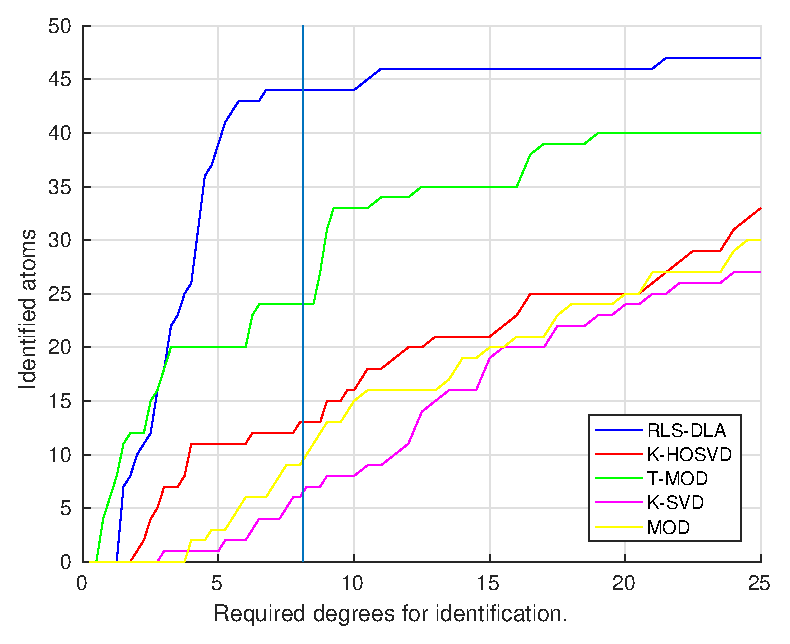
\includegraphics[width=10cm]{figures/5_20_2000_1000_100.eps}
     \caption{Cumulative atom identificatin per degree rates. $T=2000$, $M=20$, $N=50$}
     \label{fig:fig1}
\end{figure}

Figure \ref{fig:fig2} presents the results for recovering a dictionary of $M=80$ and $N=30$. It is possible to observe that the tensor-base methods outperform MOD, RLS-DLA and K-SVD in number of identified atoms and the required degrees for identification. Note that MOD performs quite silimar to RLS-DLA, while K-SVD is the worst evaluated case for this experiment. Considering the tensor-based methods, T-MOD outperforms K-HOSVD with higher atom identification over lower degrees. The experimental results verify that the tensor-based dictionary learning algorithms are able to identify more dictionary atoms when dealing with larger dictionaries and that they converge faster.

\begin{figure}[!htb]
     \centering 
	 \includegraphics[width=10cm]{figures/5_20_2000_24000_100.eps}
     \caption{Cumulative atom identificatin per degree rates. $T=2000$, $M=80$, $N=30$}
     \label{fig:fig2}
\end{figure}

The results reveals that tensor-based algorithms can perform better for dictionary recovery problems when the dictionary size increases. Since dictionary learning and reconstruction error are usually used for sparce representation classification (SRC) problems, it is possible to supose that tensor-based algorithms can improve results of classification problems, as well as can extract hidden patterns and structure in multidimensional data analytics problems.

Recent developments in science and technology have enabled the growth and availability of raw data to occur at an explosive rate. This has created an immense opportunity for knowledge discovery and data engineering research to play an essential role in a wide range of applications from daily civilian life to national security. However, the high availability of raw data increases the challenges related to big data analytics and to imbalanced data, which corresponds to data sets exhibiting significant imbalances of classes or rare events of some classes. The fundamental issue with the imbalanced learning problem is the ability of imbalanced data to significantly compromise the performance of most standard learning algorithms

A key challenge to use SC and DL for classification is how to find proper dictionaries and coefficients that highligh discriminative structure and relationships of one dataset. Therefore, we introduce a tensor-based DL method for fraud detecton from unbalanced data. Specifically, we apply a sparse representation based classification (SRC) method through learning a tensor-based dictionary and evaluate the reconstruction error for fraud classification. In this paper, we propose a tensor-based sparse representation and dictionary learning technique to analyze mobile money transactions in order to identify frauds. We propose to use tensor-based DL for learning fraudulent and legitimante data separetelly, and apply the learned dictionaries to reconstruct a test signal and classify it as fraud or ligitimate, according to the minimum reconstruction error measured by some metrics.


\section{Related Works}
\label{sec:4_relatedworks}

Compressed sensing (also known as compressive sensing, compressive sampling, or sparse sampling) is a signal processing technique for efficiently acquiring and reconstructing a signal, by finding solutions to underdetermined linear systems. This is based on the principle that, through optimization, the sparsity of a signal can be exploited to recover it from far fewer samples than required by the Shannon-Nyquist sampling theorem. There are two conditions under which recovery is possible.[1] The first one is sparsity which requires the signal to be sparse in some domain. The second one is incoherence which is applied through the isometric property which is sufficient for sparse signals.[2][3]

A common goal of the engineering field of signal processing is to reconstruct a signal from a series of sampling measurements. In general, this task is impossible because there is no way to reconstruct a signal during the times that the signal is not measured.

Around 2004, Emmanuel Candès, Terence Tao, and David Donoho proved that given knowledge about a signal's sparsity, the signal may be reconstructed with even fewer samples than the sampling theorem requires.[4][5] This idea is the basis of compressed sensing. 	https://www.wired.com/2008/03/engineers-test-highly-accurate-face-recognition/

Sparse dictionary learning is a representation learning method which aims at finding a sparse representation of the input data (also known as sparse coding) in the form of a linear combination of basic elements as well as those basic elements themselves. These elements are called atoms and they compose a dictionary. Atoms in the dictionary are not required to be orthogonal, and they may be an over-complete spanning set. This problem setup also allows the dimensionality of the signals being represented to be higher than the one of the signals being observed. The above two properties lead to having seemingly redundant atoms that allow multiple representations of the same signal but also provide an improvement in sparsity and flexibility of the representation.

sparse coding is a sparse representation of one data in the form of a linear combination of basic elements. These elements are called atoms and they compose a dictionary.

One of the key principles of dictionary learning is that the dictionary has to be inferred from the input data. The emergence of sparse dictionary learning methods was stimulated by the fact that in signal processing one typically wants to represent the input data using as few components as possible. Before this approach the general practice was to use predefined dictionaries (such as fourier or wavelet transforms). However, in certain cases a dictionary that is trained to fit the input data can significantly improve the sparsity, which has applications in data decomposition, compression and analysis and has been used in the fields of image denoising and classification, video and audio processing. Sparsity and overcomplete dictionaries have immense applications in image compression, image fusion and inpainting.

RLS-DLA \cite{skretting2010recursive}, K-SVD \cite{aharon2006rm} and MOD \cite{engan1999method}

T-MOD and K-HOSVD \cite{roemer2014tensor} 

Face recognition...

Fisher...

Florian...

Tem que ver outro...


\section{Data Model}
\label{sec:4_datamodel}

Imbalance data where zero is predominante

Data divided into learning and test, with isfraud labels with 1 or 0


The Kronecker model (\ref{eq:eq02}) can be rewritten in an equivalent tensor form. Applying the algebraic rules for unfoldings of n-mode products \cite{roemer2014tensor} we can rewrite (\ref{eq:eq02}) into a "Tucker-2" decomposition, as

\begin{equation}\label{eq:eq03}
\boldsymbol{\mathcal{X}} = \boldsymbol{\mathcal{S}} \times_1 \boldsymbol{A}^{(1)} \times_2 \boldsymbol{A}^{(2)} +  \boldsymbol{\mathcal{W}},
\end{equation}

where $\boldsymbol{\mathcal{X}} \in \mathbb{C}^{M_1 \times M_2 \times T}$, $\boldsymbol{\mathcal{S}} \in \mathbb{C}^{N_1 \times N_2 \times T}$, and $\boldsymbol{\mathcal{W}} \in \mathbb{C}^{M_1 \times M_2 \times T}$ are rearranged versions of the matrices $\boldsymbol{X}$, $\boldsymbol{S}$, and $\boldsymbol{W}$ such that $\boldsymbol{X} = [\boldsymbol{\mathcal{X}}]_{(3)}^T$, $\boldsymbol{S} = [\boldsymbol{\mathcal{S}}]_{(3)}^T$, and $\boldsymbol{W} = [\boldsymbol{\mathcal{W}}]_{(3)}^T$, respectively.

We consider a randomly generated data in order to evaluate the proposed approach, where initially $\boldsymbol{A}^{(1)}$ and $\boldsymbol{A}^{(2)}$ are gaussian distributed and randomly generated, then the dictionary $\boldsymbol{A}$ is obtained. In order to be able to evaluate the dictionary reconstruction, the sparse data $\boldsymbol{\mathcal{X}}$ is generated from the dictionary $\boldsymbol{A}$, which is used for further comparisons. We adopt 20 as the signal-to-noise ratio (snr) and 5 as the sparseness factor of the data $\boldsymbol{\mathcal{X}}$. 

The dictionary estimation is evaluated by applying the proposed approach to estimate the dictionary $\boldsymbol{A}$ from the sparse data $\boldsymbol{\mathcal{X}}$, according the selected number of sample training and iterations for the optimization problem.


\section{Proposed Approach}
\label{sec:4_proposal}

...

\section{Experiments}
\label{sec:4_experiments}

rocauc is usually used for classification evaluation, but It os not the best option for imbalance data, and Also because It does not consider the unclassified cases, such as false negatives

Receiver Operating Characteristic Curve (ROC curve) http://www.chioka.in/differences-between-roc-auc-and-pr-auc/

A ROC curve is plotting True Positive Rate (TPR) against False Positive Rate (FPR).

TPR is defined as:

tpr-formula

FPR is defined as:

fpr-formula

where TP = true positive, TN = true negative, FP = false positive, FN = false negative.

A typical ROC curve looks like this, which shows two ROC curves for Algorithm 1 and Algorithm 2.

sample-ROC-curve

The goal is to have a model be at the upper left corner, which is basically getting no false positives – a perfect classifier.

The receiver operating characteristic area under curve (ROC AUC) is just the area under the ROC curve. The higher it is, the better the model is.

Precision Recall Curve (PR Curve)
A PR curve is plotting Precision against Recall.

Precision is defined as:

precision-formula

Recall is defined as:

recall-formulaA typical PR curve looks like this, which shows two PR curves for Algorithm 1 and Algorithm 2.

sample-PR-curve

The goal is to have a model be at the upper right corner, which is basically getting only the true positives with no false positives and no false negatives – a perfect classifier.

The precision recall area under curve (PR AUC) is just the area under the PR curve. The higher it is, the better the model is.

Differences between the ROC AUC and PR AUC
Randy has given a great explanation here, plus a little of my understanding.

Since PR does not account for true negatives (as TN is not a component of either Precision or Recall), or there are many more negatives than positives (a characteristic of class imbalance problem), use PR. If not, use ROC.

Due to the inherent complex characteristics of imbalanced data sets, learning from such data requires new understandings, principles, algorithms, and tools to transform vast amounts of raw data efficiently into information and knowledge representation.

We adopt precision recall curve and compare with logistic regression based on original and pca data

Classification based on reconstruction or other value, such as similarity analysis

Evaluate what metric is more discriminative, mse, tsnr or other


\section{Conclusion}
\label{sec:4_conclusion}

The conclusion goes here.

The importance of the right metric for classification of imbalanced data

Tensor based analysis explores the extructure and relationship of multidimensional data and can improve the discriminative power of imbalanced data for classification

Can be used for feature extraction and used for well known algorithm,  and can be used for discriminative classification based on heuristics

Our proposal is better for imbalanced data than others techniques

%However, tensor-based algorithms face challenges to achieve reasonable processing time to handle large-scale tensor factorizations \cite{de2014distributed}, demanding efforts in order to explore distributed processing techniques for tensor-based analytics of large datasets. We propose a distributed and tensor-based approach for multidimensional dictionary learning in order to obtain better processing time for larger datasets. We focus on a distributed implementation of T-MOD \cite{roemer2014tensor} algorithm, based on a modification of Almeida and Kibangou's \cite{de2014distributed} approach to use Tucker-2 decomposition. We perform experiments to test different methods for learning dictionaries, evaluating the processing time and the reconstruction of a dictionary of multidimensional and separable data.